\subsection*{Función hidruro}
Son compuestos binarios que se originan de la combinación del hidrógeno con otro elemento.
\subsubsection*{Hidruro metálico}
\begin{Theorem*} {hidruro metálico}
	\begin{figure}[H]
		\centering
		\begin{tikzpicture}
			\node at (0,3) {$\text{Metal} + \mathrm{H}^{-1} \rightarrow \text{hidruro metálico}$};
			\draw[<-] (-2,2.7) -- (-2,2.5);
			\draw (-2,2.5) -- (-4,2.5);
			\draw (-4,2.5) -- (-4, 1.8);
			\draw[->] (-4,1.8) -- (-3.6, 1.8);
			\draw (-3.5,2.2) -- (-3.5, -1.2);
			\node[anchor=mid west] at (-3.5,2) {- monovalentes con +1};
			\node[anchor=mid west] at (-3.5,1.5) {- bivalentes con +2};
			\node[anchor=mid west] at (-3.5,1) {- trivalentes con +3};
			\node[anchor=mid west] at (-3.5,0.5) {- monobivalentes con +1};
			\node[anchor=mid west] at (-3.5,0) {- monotrivalentes con +1};
			\node[anchor=mid west] at (-3.5,-0.5) {- bitrivalentes con +2 +3};
			\node[anchor=mid west] at (-3.5,-1) {- bitetravalentes con +4};
		\end{tikzpicture}
	\end{figure}
	$$\ch{M^{+} + H^{-1} ->}\mathrm{M}\mathrm{H}_x$$
\end{Theorem*}
\noindent Ejemplos:
\begin{align*}
	&\ch{"\ox{+1,Au}" + "\ox{-1,H}" -> AuH} \ \text{\{ T: hidruro auroso} \\
	&\ch{"\ox{+2,Fe}" + "\ox{-1,H}" -> FeH2} \ \text{\{ T: hidruro ferroso} \\
	&\ch{"\ox{+3,Fe}" + "\ox{-1,H}" -> FeH3} \ \text{\{ T: hidruro férrico} \\
	&\ch{"\ox{+4,Sn}" + "\ox{-1,H}" -> SnH4} \ \text{\{ T: hidruro estánico} \\
	&\ch{"\ox{+1,Na}" + "\ox{-1,H}" -> NaH} \ \text{\{ T: hidruro de sodio} \\
	&\ch{"\ox{+2,Ca}" + "\ox{-1,H}" -> CaH2} \ \text{\{ T: hidruro de calcio} \\
\end{align*}
\subsubsection*{Hidruro no metálico - Aminas}
\begin{Theorem*} {Aminas}
	\begin{figure}[H]
		\centering
		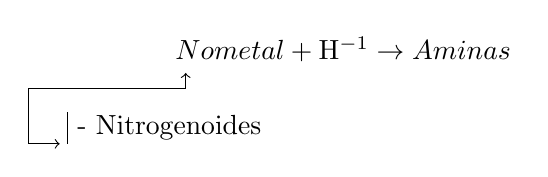
\begin{tikzpicture}
			\node at (0,3) {$\text{No metal} + \mathrm{H}^{-1} \rightarrow \text{Aminas}$};
			\draw[<-] (-2,2.7) -- (-2,2.5);
			\draw (-2,2.5) -- (-4,2.5);
			\draw (-4,2.5) -- (-4, 1.8);
			\draw[->] (-4,1.8) -- (-3.6, 1.8);
			\draw (-3.5,2.2) -- (-3.5, 1.8);
			\node[anchor=mid west] at (-3.5,2) {- Nitrogenoides};
		\end{tikzpicture}
	\end{figure}
	$$\ch{NIT^{-3} + H^{+1} ->}\mathrm{NIT}\mathrm{H}_3$$
\end{Theorem*}
\noindent Ejemplos:
\begin{align*}
	&\ch{"\ox{-3,N}" + "\ox{+1,H}" -> NH3}\left\{\begin{array}{l}
		\text{T: amina}\\
		\text{T: amoniaco}
	\end{array}\right. \\
	&\ch{"\ox{-3,P}" + "\ox{+1,H}" -> PH3}\left\{\begin{array}{l}
		\text{T: fosfamina}\\
		\text{T: fosfina}
	\end{array}\right. \\
	&\ch{"\ox{-3,As}" + "\ox{+1,H}" -> AsH3}\left\{\begin{array}{l}
		\text{T: arsenamina}
	\end{array}\right. \\
	&\ch{"\ox{-3,Sb}" + "\ox{+1,H}" -> SbH3}\left\{\begin{array}{l}
		\text{T: estivamina}\\
		\text{T: estibina}
	\end{array}\right. \\
	&\ch{"\ox{-3,B}" + "\ox{+1,H}" -> BH3}\left\{\begin{array}{l}
		\text{T: boramina}
	\end{array}\right.
\end{align*}
\subsubsection*{Hidruro no metálico - Silanos}
\begin{Theorem*} {Silanos}
	\begin{figure}[H]
		\centering
		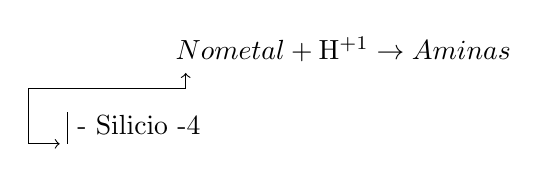
\begin{tikzpicture}
			\node at (0,3) {$\text{No metal} + \mathrm{H}^{+1} \rightarrow \text{Aminas}$};
			\draw[<-] (-2,2.7) -- (-2,2.5);
			\draw (-2,2.5) -- (-4,2.5);
			\draw (-4,2.5) -- (-4, 1.8);
			\draw[->] (-4,1.8) -- (-3.6, 1.8);
			\draw (-3.5,2.2) -- (-3.5, 1.8);
			\node[anchor=mid west] at (-3.5,2) {- Silicio -4};
		\end{tikzpicture}
	\end{figure}
	$$\ch{Si + H^{+1} ->}\mathrm{Si}_n\mathrm{H}_{2n+2}$$
\end{Theorem*}
\noindent Ejemplos:
\begin{align*}
	&n=1 \ \ch{SiH4}\left\{\begin{array}{l}
		\text{T: silano}
	\end{array}\right. \\
	&n=2 \ \ch{Si2H6}\left\{\begin{array}{l}
		\text{T: disilano}
	\end{array}\right. \\
	&n=3 \ \ch{Si3H8}\left\{\begin{array}{l}
		\text{T: trisilano}
	\end{array}\right. \\
	&n=9 \ \ch{Si9H20}\left\{\begin{array}{l}
		\text{T: nonasilano}
	\end{array}\right.
\end{align*}
\subsubsection*{Hidruro no metálico - Ácidos hidrácidos}
\begin{Theorem*} {Ácidos hidrácidos}
	\begin{figure}[H]
		\centering
		\begin{tikzpicture}
			\node at (0,3) {$\mathrm{H}^{+1} + \text{No metal} \rightarrow \text{Ácido hidrácido}$};
			\draw[<-] (-2,2.7) -- (-2,2.5);
			\draw (-2,2.5) -- (-4,2.5);
			\draw (-4,2.5) -- (-4, 1.8);
			\draw[->] (-4,1.8) -- (-3.6, 1.8);
			\draw (-3.5,2.2) -- (-3.5, 1.3);
			\node[anchor=mid west] at (-3.5,2) {- Halógenos -1};
			\node[anchor=mid west] at (-3.5,1.5) {- Anfígenos -2};
		\end{tikzpicture}
	\end{figure}
	$$\ch{H^{+1} + NM^{-} ->}\mathrm{H}_x\mathrm{NM}$$
\end{Theorem*}
\noindent Ejemplos:
\begin{align*}
	&\ch{"\ox{+1,H}" + "\ox{-1,F}" -> HF}\left\{\begin{array}{l}
		\text{T(liq): ácido fluorhídrico} \\
		\text{T(gas): fluoruro de hidrógeno}
	\end{array}\right. \\
	&\ch{"\ox{+1,H}" + "\ox{-1,Cl}" -> HCl}\left\{\begin{array}{l}
		\text{T(liq): ácido clorhídrico} \\
		\text{T(gas): cloruro de hidrógeno}
	\end{array}\right. \\
	&\ch{"\ox{+1,H}" + "\ox{-1,Br}" -> HBr}\left\{\begin{array}{l}
		\text{T(liq): ácido bromhídrico} \\
		\text{T(gas): bromuro de hidrógeno}
	\end{array}\right. \\
	&\ch{"\ox{+1,H}" + "\ox{-1,I}" -> HI}\left\{\begin{array}{l}
		\text{T(liq): ácido yodhídrico} \\
		\text{T(gas): yoduro de hidrógeno}
	\end{array}\right. \\
	&\ch{"\ox{+1,H}" + "\ox{-2,S}" -> H2S}\left\{\begin{array}{l}
		\text{T(liq): ácido sulfhídrico} \\
		\text{T(gas): sulfuro de hidrógeno}
	\end{array}\right. \\
	&\ch{"\ox{+1,H}" + "\ox{-2,Se}" -> H2Se}\left\{\begin{array}{l}
		\text{T(liq): ácido selenhídrico} \\
		\text{T(gas): selenuro de hidrógeno}
	\end{array}\right. \\
	&\ch{"\ox{+1,H}" + "\ox{-2,Te}" -> H2Te}\left\{\begin{array}{l}
		\text{T(liq): ácido telurhídrico} \\
		\text{T(gas): teluro de hidrógeno}
	\end{array}\right. \\
\end{align*}